\chapter{Appendix}

\section*{Supplementary Materials}

\vspace{15pt}
\renewcommand\thesection{\Alph{section}.}
\renewcommand\thesubsection{\Alph{section}.\arabic{subsection}}
\setcounter {subfigure} {0}
\setcounter {figure} {0}
\setcounter {section} {0}
\setcounter {page} {1}

\section{Multiplexing $M+N$ Iterator Executions for Maximizing Pipeline Utilization}

We claimed in \S\ref{ssec:architecture} that if $t_c = \eta \cdot t_d$ for all offloaded iterator executions, it is always possible to multiplex $m + n$ concurrent iterator executions and fully utilize all memory and logic pipelines. We prove our claim by providing a staggered scheduling algorithm (Algorithm~\ref{alg:scheduling}) that ensures such multiplexing across $m+n$ iterator executions. The scheduler processes $m+n$ iterator execution requests, assigning each a memory pipeline, a logic pipeline, and staggered start times. These requests are then executed in the respective memory pipelines. Through this staggered scheduling approach, \name fully utilizes the $n$ memory pipelines and $m$ logic pipelines, ensuring no resources are wasted. Note that this algorithm is a simplified version to illustrate the potential for full pipeline saturation under the given condition. \name's scheduler implements a real-time algorithm to multiplex incoming requests on the fly.


\begin{algorithm}
\caption{Staggered-Scheduling}
\label{alg:scheduling}
\begin{algorithmic}[1]
\State $m, n \gets$ number of logic, memory pipelines
\State $L_i, M_j \gets$ $i^{th}$ logic pipeline, $j^{th}$ memory pipeline
\State $t_d \gets$ data fetch time per pointer traversal iteration

\While{true}
    %\State Increment $clock$
    \State Dequeue $n + m$ requests from network stack
    \For{$i \gets 1$ \textbf{to} $m + n$}
        \State Assign request $R_i$ to ($M_{i \bmod n}$,  $L_{i \bmod m}$)
        \State Schedule $R_i$ to start at time $(i-1) \cdot \frac{t_d}{n}$
        
        
    \EndFor
    
    \State Start requests as scheduled at memory pipelines
    
\EndWhile
\end{algorithmic}
\end{algorithm}


\subsection{\name Empirical Analysis}
Prior studies have shown that real-world data-centric cloud applications spend a significant fraction of time traversing pointers, as summarized in Fig.~\ref{fig:sup_motivation}.

\begin{figure}[b]
    \centering
    \footnotesize
     \subfigure[Survey from prior studies]{
                \begin{tabular}[b]{c|c} 
                    \textbf{Application} & \specialcell{\textbf{\% of time spent}\\\textbf{in pointer traversal}} \\ \hline
                    GraphChi~\cite{graphchi} & $\sim 93\%$ \\ \hline
                    MonetDB\cite{monetdb} & $70\%-97\%$ \\ \hline
                    GC in Spark~\cite{spark} & $\sim 72$\% \\ \hline
                    VoltDB~\cite{voltdb} & Up to $49.55$\% \\ \hline
                    MemC3~\cite{memc3} & Up to $21.15$\% \\ \hline
                    DBx1000 \cite{db1000} & $\sim 9$\% \\\hline
                    Memcached\cite{memcached} & $\sim 7$\% \\ \hline\hline
                \end{tabular} 
    }
            \label{tab:sup_motivation}
    \vspace{-1em}
    \caption{\textbf{Time cloud applications spend in pointer traversals} based on prior studies}
    \label{fig:sup_motivation}%\vspace{-1.5em}
\end{figure}

\section{\name Supported Data Structures}
\label{sec:appendix}



We adapt $13$ data structures across $4$ popular open-sourced libraries to \name's iterator abstraction (\S\ref{sec:interface}). In particular, we outline how the data structure implementations for certain operations can be expressed using \code{init()}, \code{next()}, and \code{end()}. For simplicity and readability, (i) we assume that the data structure developer defines a macro, \code{SP\_PTR\_(variable\_name)}, as the address of the variable resides on the \code{scratch\_pad}, and (ii) we omit obvious type conversions for de-referenced pointers. 

We analyze two widely used categories of data structures: lists and trees. In our analysis, we find that the top-level data structure APIs (\ie, the APIs used by applications) use the same base function under the hood. For instance, list and forward list in the STL library share the same internal function, \code{std::find()}. We summarize our findings in Table \ref{table:extra-apps-2}, including the data structure libraries, their category, the top-level data structure APIs, and the internal base function.

\paragraphb{List structures} Our surveyed list structures already follow the execution flow of \name iterator: \code{init()}, \code{next()}, and \code{end()}.

These data structures generally have compute-intensive \code{end()} functions to check multiple termination conditions, while their \code{next()} function simply dereferences a single pointer to the next node. Listing \ref{lst:list} and Listing \ref{lst:list_mod} demonstrate a linked list with two termination conditions: (i) value is found or (ii) search reaches the end. To indicate which condition is met, a special flag (\eg, \code{KEY\_NOT\_FOUND}) is written on the \code{scratch\_pad}. Listing~\ref{lst:bimap} and Listing~\ref{lst:bimap_mod} describe a bitmap that uses a hashtable internally, where colliding entries are stored in linked lists within the same bucket. As such, the \name iterator interface resembles that of \code{std::list} quite closely.

\paragraphb{Tree-like data structures}
Compared to list structures, tree data structures require more computation in the \code{next()} function, as the next pointer is determined based on the value in the child node. For instance, in \code{Btree} (Listing \ref{lst:btree}, \ref{lst:btree_mod}), the next function iterates through internal node keys, comparing them to the search key. Interestingly, \code{std::map} (Listing \ref{lst:map}, \ref{lst:map_mod}) and Boost AVL trees (Listing \ref{lst:avltree}, \ref{lst:avltree_mod}) share the same offload function structure, with only minor implementation and naming differences.

\begin{table*}[!h]
  \centering
  % \renewcommand{\arraystretch}{0.95}
  \captionof{table}{\small Additional data structure supported by \name.}
  \vspace{-1em}
  \scriptsize
  \begin{tabular}{L{.12\textwidth}|L{.06\textwidth}|L{.05\textwidth}|L{.22\textwidth}|L{.22\textwidth}|L{.09\textwidth}|L{.07\textwidth}}
    \hline
    {\bf Data Structure} & {\bf Category} & {\bf Library} & {\bf Data structure API} & {\bf Internal function} & {\bf Original code} & {\bf \name code}\\\hline
    \hline
    List & \multirow{5}{*}{List} & \multirow{2}{*}{STL} & \multirow{2}{*}{\texttt{std::find(start, end, value)}} & \multirow{2}{*}{\texttt{std::find(start, end, value)}} &\multirow{2}{*}{Listing~\ref{lst:list}} & \multirow{2}{*}{Listing~\ref{lst:list_mod}}  \\\cline{1-1}
    Forward list & & &  & & & \\\cline{1-1}\cline{3-7}
    Bimap &  & \multirow{3}{*}{Boost} &  \multirow{3}{*}{\texttt{find(key, hash)}} & \multirow{3}{*}{\texttt{find(key, hash)}} &\multirow{3}{*}{Listing \ref{lst:bimap}} & \multirow{3}{*}{Listing \ref{lst:bimap_mod}}\\\cline{1-1}
    Unordered map  &  &  &  &  & & \\\cline{1-1}
    Unordered set  &  &  &  &  & & \\\hline
    Btree & \multirow{8}{*}{Tree} & Google & \multirow{8}{*}{\texttt{find(\&key)}} & \makecell[l]{\texttt{internal\_locate\_plain}\\\texttt{\_compare(key, iter)}} & Listing \ref{lst:btree} & Listing \ref{lst:btree_mod}\\\cline{1-1}\cline{3-3}\cline{5-7}
    Map & & \multirow{4}{*}{STL} & & \multirow{4}{*}{\texttt{\_M\_lower\_bound(x, y, key)}} &\multirow{4}{*}{Listing \ref{lst:map}} & \multirow{4}{*}{Listing \ref{lst:map_mod}}\\\cline{1-1}
    Set & & & & &  & \\\cline{1-1}
    Multimap & & & & & & \\\cline{1-1}
    Multiset & & & & & & \\\cline{1-1}\cline{3-3}\cline{5-7}
    AVL tree & & \multirow{3}{*}{Boost} & & \multirow{3}{*}{\texttt{lower\_bound\_loop(x, y, key)}} &\multirow{3}{*}{Listing \ref{lst:avltree}} & \multirow{3}{*}{Listing~\ref{lst:avltree_mod}}\\\cline{1-1}
    Splay tree & & & & & & \\\cline{1-1}
    Scapegoat tree & & & & & & \\
    \hline
  \end{tabular}
  \label{table:extra-apps-2}
\end{table*}
\setcounter {lstlisting} {0}
\setcounter {table} {1}



% STL
\lstset{frame=tb,
  xleftmargin=0cm,
  linewidth=0.95\textwidth
}
\captionsetup[lstlisting]{style=centered_lstlisting}

\vspace{2em}

\begin{minipage}{0.47\textwidth}
\subsection{List data structure in STL library}
\centering
\begin{lstlisting}[caption={C++ STL realization for \code{std::find()}},label={lst:list}, captionpos=t]
struct node {
    value_type value;
    struct node* next;
};

node* find(node* first, node* last, const value_type& value)
{
    for (; first != last; first=first->next)
        if (first->value == value)
            return first;
    return last;
}
\end{lstlisting}

\begin{lstlisting}[caption={\name realization for \code{std::find()}},label={lst:list_mod}, captionpos=t]
class list_find : chase_iterator {

    init(void *value, void* first) {
        *SP_PTR_VALUE = value;
        cur_ptr = first;
    }
  
    void* next() {
        return cur_ptr->next;
    }
  
    bool end() {
        if (*SP_PTR_VALUE == cur_ptr->value) {
            *SP_PTR_RETURN = cur_ptr;  
            return true;
        }
        if (cur_ptr->next == NULL) {
            *SP_PTR_RETURN = KEY_NOT_FOUND;  
            return true;
        }
        return false;
    }
}
\end{lstlisting}
% \vspace{-20pt}
\end{minipage}

%\vspace{10cm}

\begin{minipage}{0.47\textwidth}
\subsection{List data structure in Boost library}
\centering
% \vspace{-5pt}
\begin{lstlisting}[caption={Boost realization for \code{bimap::find()}},label={lst:bimap}, captionpos=t]
struct node {
    key_type key;
    struct node* next;
    value_type value;
};
void* find(const key_type& key, const hash_type& hash) const
{
    // The bucket start pointer can be pre-computed before offloading
    std::size_t buc = buckets.position(hash(key));
    node_ptr start = buckets.at(buc)
    for(node_ptr x = start; x != NULL; x = x->next){
        if(key == x->key){
            return x;
        }
    }
    return NULL;
}
\end{lstlisting}

\begin{lstlisting}[caption={\name realization for \code{bimap::find()}},label={lst:bimap_mod}, captionpos=t]
class bimap_find : chase_iterator {
public:
    key_type key;
  
    init(void *key, void* start) {
        *SP_PTR_KEY = key;
        cur_ptr = start;
    }
  
    void* next() {
        return cur_ptr->next;
    }
  
    bool end() {
        if (*SP_PTR_KEY == cur_ptr->key) {
            *SP_PTR_RETURN = cur_ptr;
            return true;
        }
        if (cur_ptr->next == NULL) {
            *SP_PTR_RETURN = NULL;  
            return true;
        }
        return false;
    }
}
\end{lstlisting}
% \vspace{-20pt}
\end{minipage}

\begin{minipage}{0.47\textwidth}
\subsection{Tree data structure in Google library}
\centering
% \vspace{-5pt}
\begin{lstlisting}[caption={Google realization for\\\code{btree::internal\_locate\_plain\_compare()}},label={lst:btree}, captionpos=t]
#define kNodeValues 8
struct btree_node {
    bool is_leaf;    
    int num_keys;
    key_type keys[kNodeValues];
    btree_node* child[kNodeValues + 1];
};
IterType btree::internal_locate_plain_compare(const key_type &key, IterType iter) const {
    for (;;) { 
        int i;
        for(int i = 0; i < iter->num_keys; i++) {
            if(key <= iter->keys[i]) {
                break;
            }
        }
        if (iter.node->is_leaf) {
            break;
        }
        iter.node = iter.node->child(i);
    }
    return iter;
}
\end{lstlisting}

\begin{lstlisting}[caption={\name realization for\\\code{btree::internal\_locate\_plain\_compare()}},label={lst:btree_mod}, captionpos=t]
class btree_find_unique : chase_iterator {
    init(void *key, void* iter) {
        *SP_PTR_KEY = key;
        cur_ptr = iter;
    }
  
    void* next() {
        *SP_PTR_I = 0;
        for(; *SP_PTR_I < cur_ptr->num_keys; *SP_PTR_I++) {
            if(*SP_PTR_KEY <= cur_ptr->keys[*SP_PTR_I]) 
            {
                break;
            }
        }
        cur_ptr = cur_ptr->child[*SP_PTR_I];
    }
  
    bool end() {
        if(cur_ptr->is_leaf) {
            *SP_PTR_RETURN = cur_ptr;
            return true;
        } else {
            return false;
        }
    }
}
\end{lstlisting}
% \vspace{-20pt}
\end{minipage}




% Google



\begin{comment}
\begin{center}
\centering
% \vspace{-5pt}
\begin{lstlisting}[caption={Google LevelDB realization for \code{Skiplist::find()}},label={lst:skiplist}, captionpos=t]
struct SkipListNode {
    key_type key;
    SkipListNode* next_[1];
};
SkipListNode* FindGreaterOrEqual(const Key& key, Node** prev) const {
    Node* x = head_;
    int level = max_height_ - 1;
    while (true) {
        if (x->next_[level] != NULL && key < x->next_[level]->key) {
            // Keep searching in this list
            x = x->next_[level];
        } else {
            if (prev != nullptr) prev[level] = x;
            if (level == 0) {
                return x->next_[level];
            } else {
                // Switch to next list
                level--;
            }
        }
    }
}
\end{lstlisting}
% \vspace{-10pt}
\begin{lstlisting}[caption={\name realization for \code{Skiplist::find()}},label={lst:skiplist_mod}, captionpos=t]
class skiplist_find : chase_iterator {
  
    init(void* key, void* head_, void* prev, int level) {
        *SP_PTR_KEY = key;
        cur_ptr = head_;
        *SP_PTR_PREV = prev;
        *SP_PTR_LEVEL = level;
        *SP_PTR_RETURN = NULL;
    }
  
    void* next() {
        return cur_ptr->next_[*SP_PTR_LEVEL];
    }
  
    bool end() {
        if (x->next_[*SP_PTR_LEVEL] != NULL && key < x->next_[*SP_PTR_LEVEL]->key) {
            return false;   
        } else {
            if (*SP_PTR_PREV != NULL) *SP_PTR_PREV[*SP_PTR_LEVEL] = x;
            if (*SP_PTR_LEVEL == 0) {
                *SP_PTR_RETURN = x->next_[*SP_PTR_LEVEL];
                return true;
            } else {
                // Switch to next list
                *SP_PTR_LEVEL--;
                return false;
            }
        }
    }
}
\end{lstlisting}
% \vspace{-20pt}
\end{center}

\end{comment}


\begin{minipage}{0.47\textwidth}
\subsection{Tree data structure in STL library}
\centering
% \vspace{-5pt}
\begin{lstlisting}[caption={C++ STL realization for \code{map::find()}},label={lst:map}, captionpos=t]
struct node {
    key_type key;
    node* left;
    node* right;
};

_M_lower_bound(node* x, node* y, const key_type& key)
{
    while (x != 0) {
        if (x->key <= key) {
            y = x; 
            x = x->left;
        } else {
            x = x->right;
        }
    }
    return y;
}
\end{lstlisting}

\begin{lstlisting}[caption={\name realization for \code{map::find()}},label={lst:map_mod}, captionpos=t]
class map_find : chase_iterator {
    init(void *key, void* x, void* y) {
        *SP_PTR_KEY = key;
        *SP_PTR_Y = y;
        cur_ptr = x;
    }
  
    void* next() {
        if (cur_ptr->key <= *SP_PTR_KEY) {
            *SP_PTR_Y = cur_ptr;  
            cur_ptr = cur_ptr->left;
        } else {
            cur_ptr= cur_ptr->right;
        }
        return cur_ptr->left;
    }
  
    bool end() {
        if (cur_ptr == NULL) {
            *SP_PTR_RETURN = *SP_PTR_Y;  
            return true;
        } else {
            return false;
        }
    }
}
\end{lstlisting}
% \vspace{-20pt}
\end{minipage}

% Boost
\begin{minipage}{0.47\textwidth}
\subsection{Tree data structure in Boost library}
\centering
% \vspace{-5pt}
\begin{lstlisting}[caption={Boost realization for \code{avltree::find()}},label={lst:avltree}, captionpos=t]
static node_ptr lower_bound_loop
(node_ptr x, node_ptr y, const KeyType &key)
{
    while(x){
        if(x->key >= key)) {
            x = x->right;
        }
        else{
            y = x;
            x = x->left;
        }
    }
    return y;
}
\end{lstlisting}

\begin{lstlisting}[caption={\name realization for \code{avltree::find()}},label={lst:avltree_mod}, captionpos=t]
class avltree_find : chase_iterator {
public:
    key_type key;
    void* y;
  
    init(void *key, void* x, void* y) {
        *SP_PTR_KEY = key;
        *SP_PTR_Y = y;
        cur_ptr = x;
    }
  
    void* next() {
        if(cur_ptr->key >= *SP_PTR_KEY) {
            cur_ptr = cur_ptr->right;
        }
        else{
            *SP_PTR_Y = cur_ptr;
            cur_ptr = cur_ptr->left;
        }
    }
  
    bool end() {
        // The result is already stored at SP_PTR_Y
        if(cur_ptr == NULL) {
            return true;
        } else {
            return false;
        }
    }
}
\end{lstlisting}
% \vspace{-20pt}
\end{minipage}

\section{\name Additional Evaluation Results}
\label{sec:appendix}

In this section, we provide additional evaluation results for \name.



\begin{figure*}[t]
\centering
  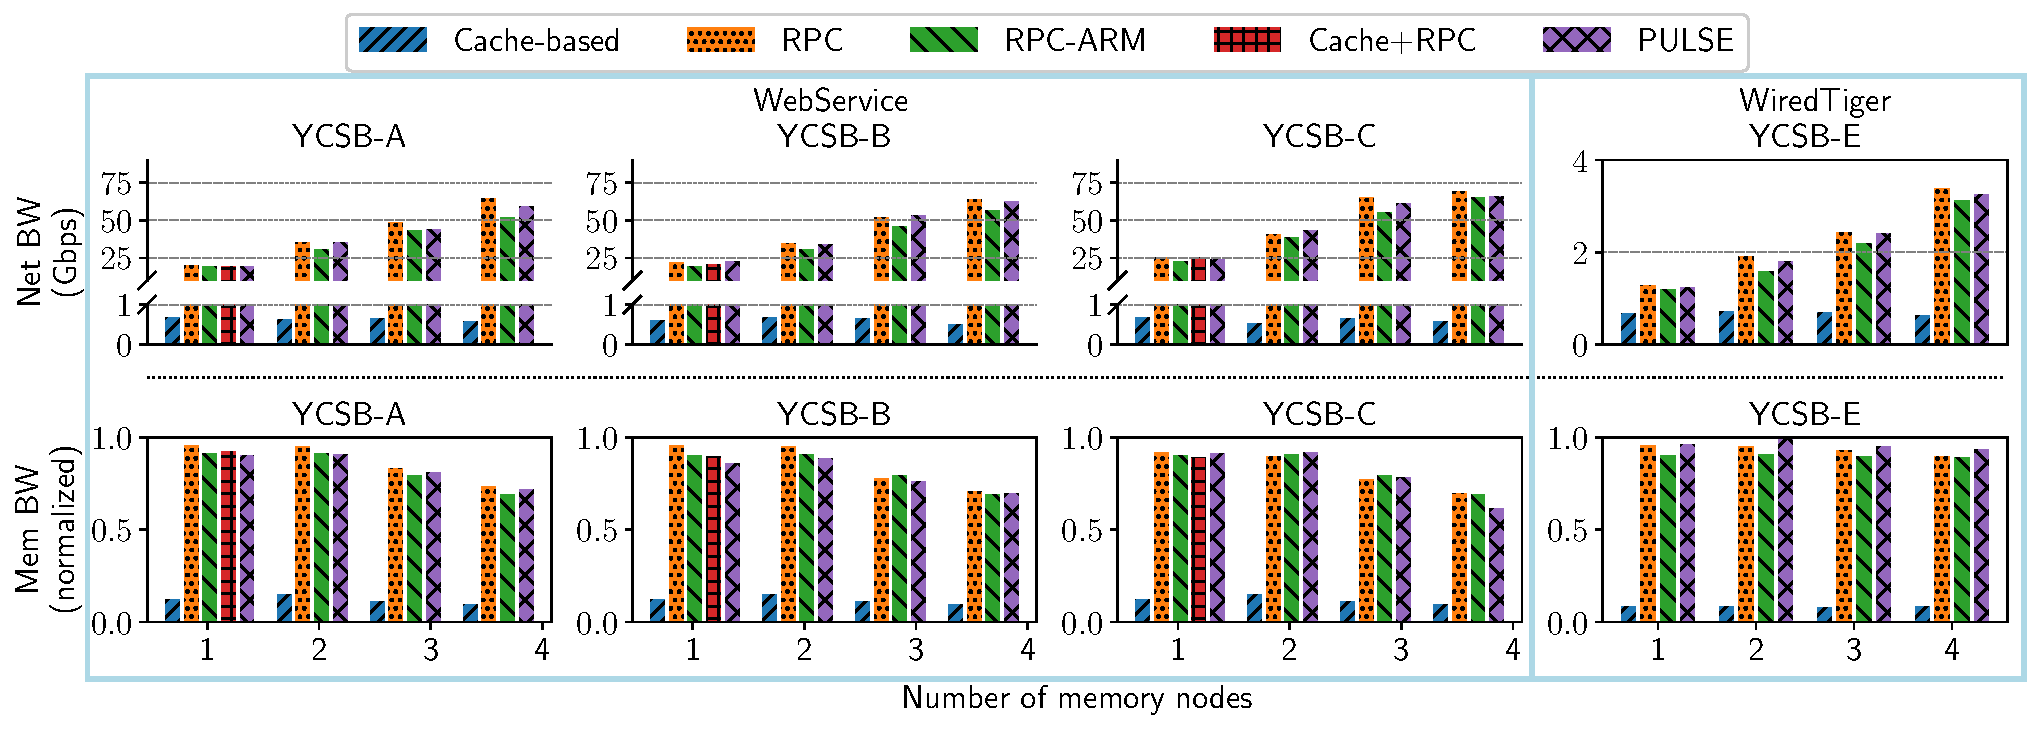
\includegraphics[width=\textwidth]{fig/pulse/network_memory.pdf}
  %\vspace{-2.5em}
  \vspace{-2.5em}
  \caption{\textbf{Network and memory bandwidth utilization.} \name and RPC utilize over 90\% of the available memory bandwidth, while the cache-based approach suffers from swap system overhead. In Webservice, the network bandwidth becomes the bottleneck due to large 8 KB data transfers.}
  % 
  % partitioning for UPC (no distributed ptr-chasing)
\label{fig:sup_eval_perf_e2e_utilization}\vspace{-2em}
\end{figure*}

\subsection{Traditional Core Architecture vs. \name} 
We evaluate the impact of the \name architectural design (\S\ref{sec:accelerator}) by comparing \name against \namearch, an in-order processor built on \name's components. We denote \textit{C\_x} as in tightly-coupled core architecture, where \textit{x} is the number of cores. We denote \textit{P\_x\_y} as \name architecture, where \textit{x} is the number of logic pipelines and \textit{y} is the number of memory pipelines. Table \ref{table:sup_architecture} shows the power, performance, and area usage of various configurations. The performance metrics are obtained by executing the WebService application with various configurations. In \name's disaggregated architecture, when the number of logic and memory pipelines is equal to that of a traditional core architecture, power and area usage are higher due to additional logic and buffering in the interconnect and scheduler. However, due to the nature of pointer traversal operations (\S\ref{sec:accelerator}), \name requires fewer logic pipelines to achieve similar performance. For example, to fully saturate the memory bandwidth of a single node, \name uses only one logic pipeline and four memory pipelines, while a traditional core architecture requires four cores. As a result, \name saves 20.12\% in power with only a 7.2\% latency overhead, primarily due to the additional scheduler and data movement between workspaces.

\begin{table}[ht]
\centering
\vspace{0.5em}
\scriptsize % Sets the font size to small to fit the table in a single column
\begin{tabularx}{\columnwidth}{@{}Xcccccc@{}} % Adjust column types as needed
\toprule
\textbf{Config} & \textbf{Pwr (W)} & \textbf{LUT \%} & \textbf{BRAM \%}  & \textbf{Tpt (Mops/s)}   & \textbf{Lat (us)} \\
\midrule
C\_1 & 67.76 & 14.73 & 14.57 & 0.41 & 33.25   \\
C\_2 & 75.47 & 20.46 & 18.73 & 0.63 & 33.73   \\
C\_3 & 84.57 & 28.66 & 31.83 & 0.87 & 34.66   \\
C\_4 & 89.77 & 37.10 & 34.17 & 1.20 & 35.11  \\
P\_1\_1 & 56.74 & 11.76 & 16.34 & 0.51 & 37.57 \\
P\_1\_2 & 59.47 & 14.87 & 18.38 & 0.73 & 36.74 \\
P\_1\_3 & 64.78 & 16.64 & 22.37 & 1.01 & 38.46 \\
P\_1\_4 & 72.47 & 18.37 & 25.84 & 1.24 & 38.37 \\
P\_2\_1 & 67.37 & 17.73 & 20.37 & 0.48 & 40.27 \\
P\_2\_2 & 77.37 & 21.38 & 22.38 & 0.76 & 39.47 \\
P\_2\_3 & 81.21 & 26.22 & 26.76 & 0.99 & 41.37 \\
P\_3\_3 & 86.15 & 37.21 & 30.12 & 1.03 & 40.98 \\
P\_2\_4 & 83.21 & 30.13 & 31.21 & 1.19 & 40.37 \\
P\_4\_4 & 95.64 & 46.42 & 39.84 & 1.21 & 41.47\\
\bottomrule
\end{tabularx}
\caption{Comparison between traditional core architecture and \name architecture.}
\vspace{-2em}
\label{table:sup_architecture}
\end{table}




\begin{figure}[t]
\centering
%\vspace{-1.5em}
\subfigure[Impact of access pattern]{
  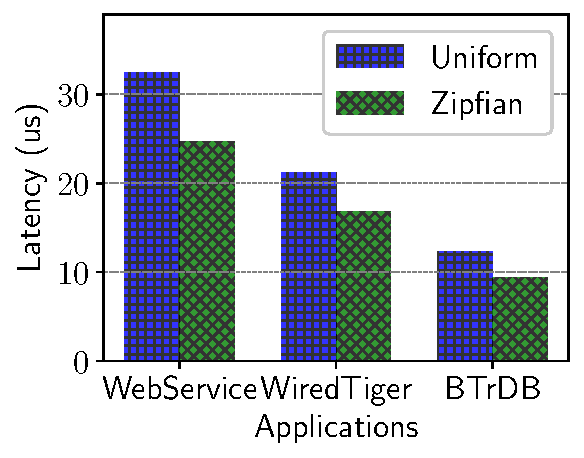
\includegraphics[width=0.45\columnwidth]{fig/pulse/micro_cache_friendly.pdf}
  \label{fig:sup_cache_friendly}}
\subfigure[Impact of modifications]{
  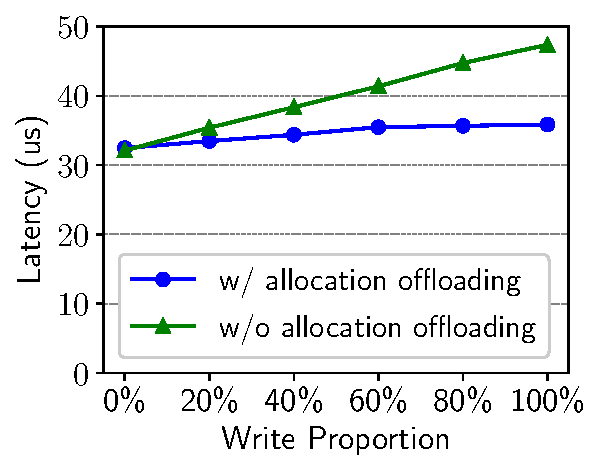
\includegraphics[width=0.45\columnwidth]{fig/pulse/micro_write.pdf}
  \label{fig:sup_write}}\vspace{-1em}
\caption{(a) \name latency is up to $1.3\times$ lower for skewed than uniform access patterns due to caching. (b) Offloaded allocations in \name improve the WebService request latencies as the proportion of writes increases by reducing the number of round trips per allocation.}
\vspace{-1.5em}
\label{fig:sup_eval_cache_friendly}
\end{figure}

\begin{figure}[!ht]
    \centering
    \subfigure[Traversal length]{
        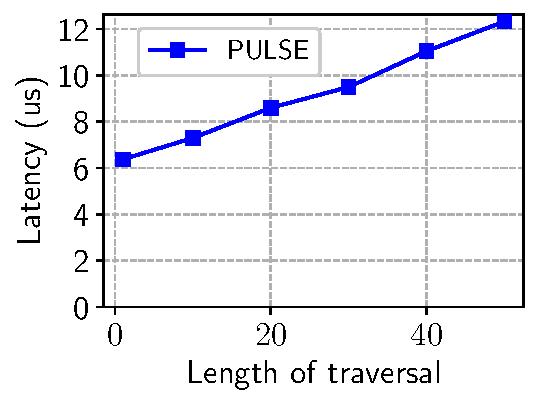
\includegraphics[width=0.45\columnwidth]{fig/pulse/sensitivity_length.pdf}
        \label{fig:sup_eval_sensitivity_length}    
    }%
    \subfigure[Number of memory pipelines]{
        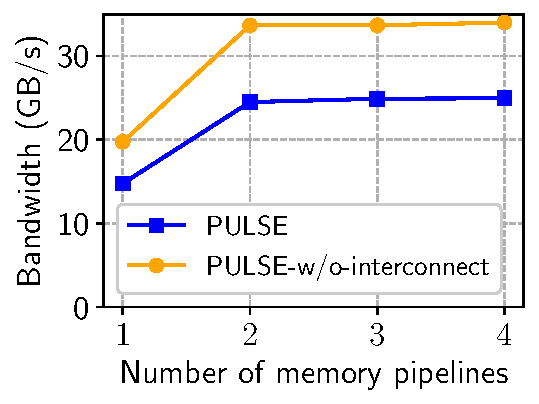
\includegraphics[width=0.45\columnwidth]{fig/pulse/sensitivity_core.pdf}
        \label{fig:sup_eval_sensitivity_core}
    }
   % \vspace{-10pt}
    \caption{\textbf{Sensitivity to traversal length and the number of memory pipelines.} (a) \name latency scales linearly with the length of traversal. (b) \name accelerator can saturate memory bandwidth with just two \name memory pipelines.}
\end{figure}
    

\begin{figure}[b]
\centering
  \vspace{-0.2em}
  \subfigure[Latency]{
    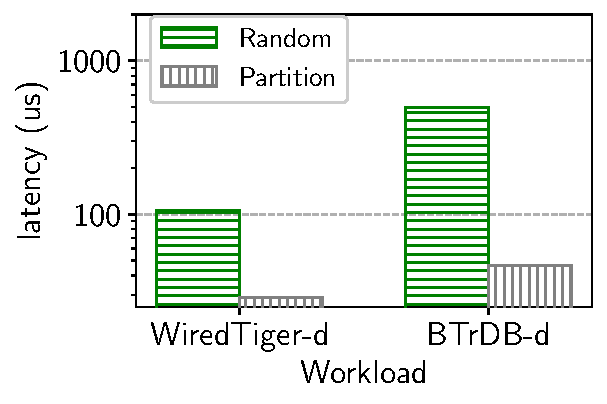
\includegraphics[width=0.45\columnwidth]{fig/pulse/sensitivity_allocation_latency.pdf}
    \label{fig:sup_eval_sensitivity_allocation_latency}
  }%
  \subfigure[Throughput]{
    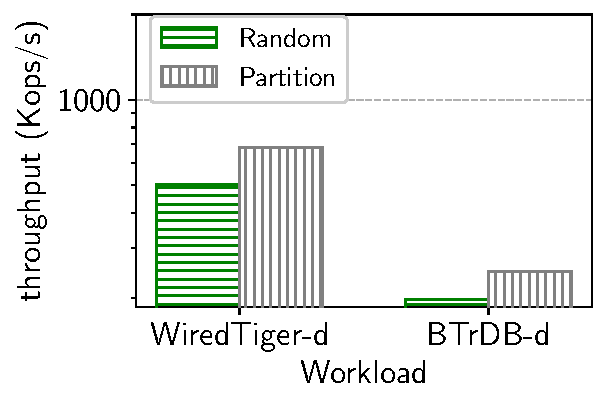
\includegraphics[width=0.45\columnwidth]{fig/pulse/sensitivity_allocation_throughput.pdf}
    \label{fig:sup_eval_sensitivity_allocation_throughput}
  }%
  %\vspace{-10pt}
  \caption{\textbf{Allocation policy.} \name performs better with the partitioned allocation since it minimizes cross-node traversals.}
\end{figure}


\subsection{Network and Memory Bandwidth Utilization} 
We evaluate the network and memory bandwidth utilization of the three applications in Fig. \ref{fig:sup_eval_perf_e2e_utilization}. For WiredTiger, \name and RPC utilize over 90\% of the available memory bandwidth, while the Cache-based approach suffers from low network bandwidth and memory utilization due to swap system overhead. For WebService, the large 8 KB data transfers saturate the maximum bandwidth that the DPDK stack can sustain~\cite{erpc}. As a result, network bandwidth becomes the bottleneck, reducing \name and RPC memory bandwidth utilization under 3 and 4 memory nodes. The memory bandwidth is normalized, where $1.0$ corresponds to $25$ GB/s per node.



\begin{figure*}[t]
\centering
  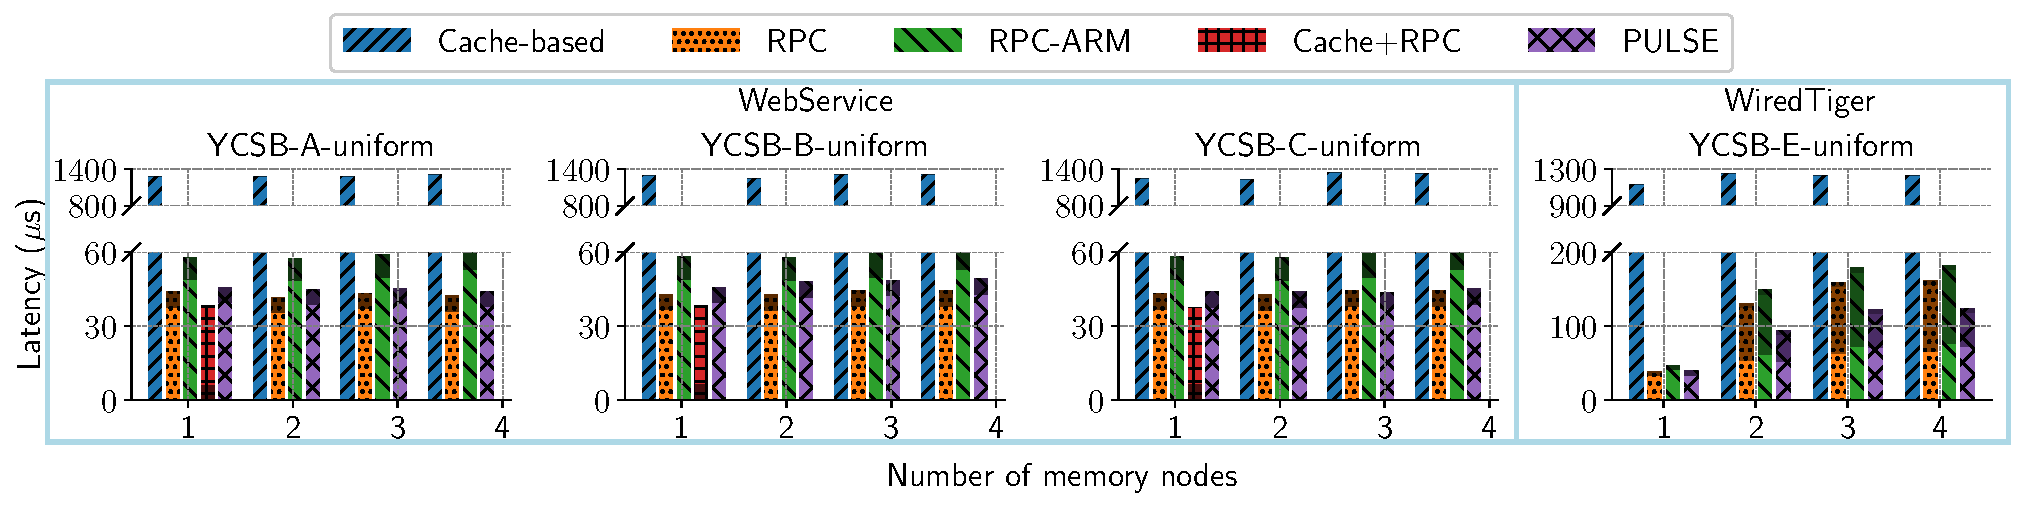
\includegraphics[width=0.9\textwidth]{fig/pulse/latency_uniform.pdf}\vspace{-.5em}
  \label{fig:sup_eval_perf_e2e_latency_uniform}
  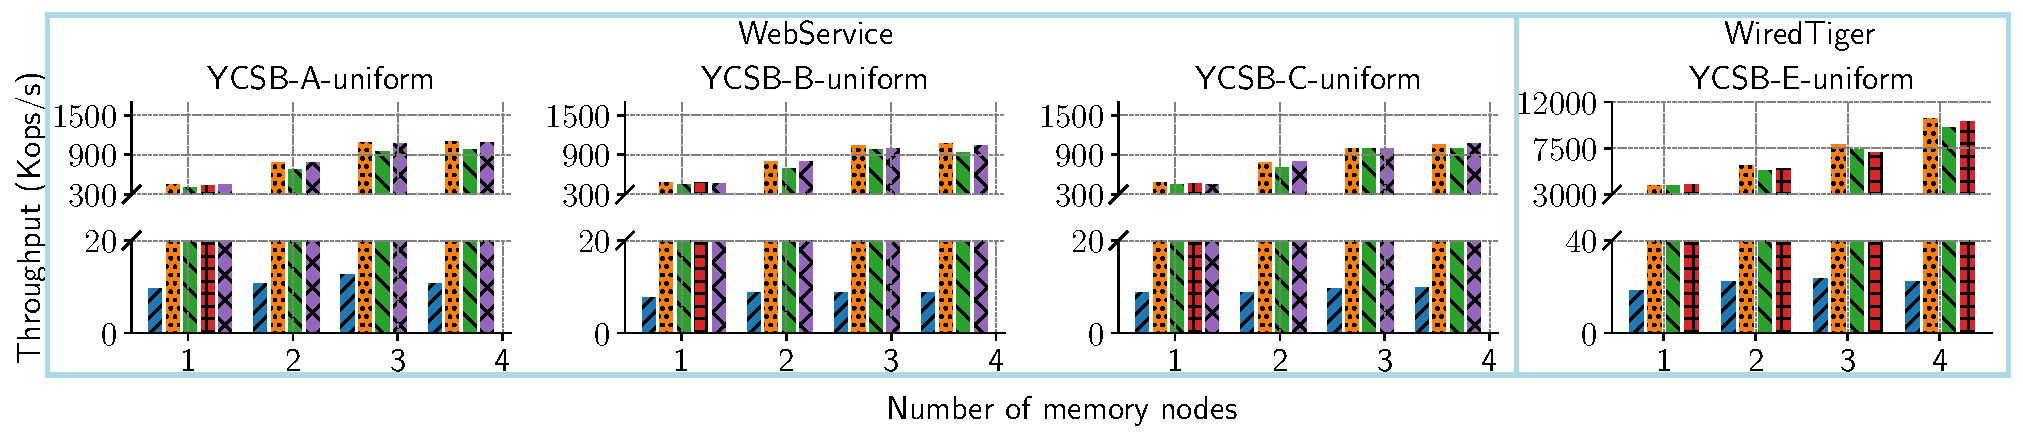
\includegraphics[width=0.9\textwidth]{fig/pulse/throughput_uniform.pdf}
  \label{fig:sup_eval_perf_e2e_throughput_uniform}
  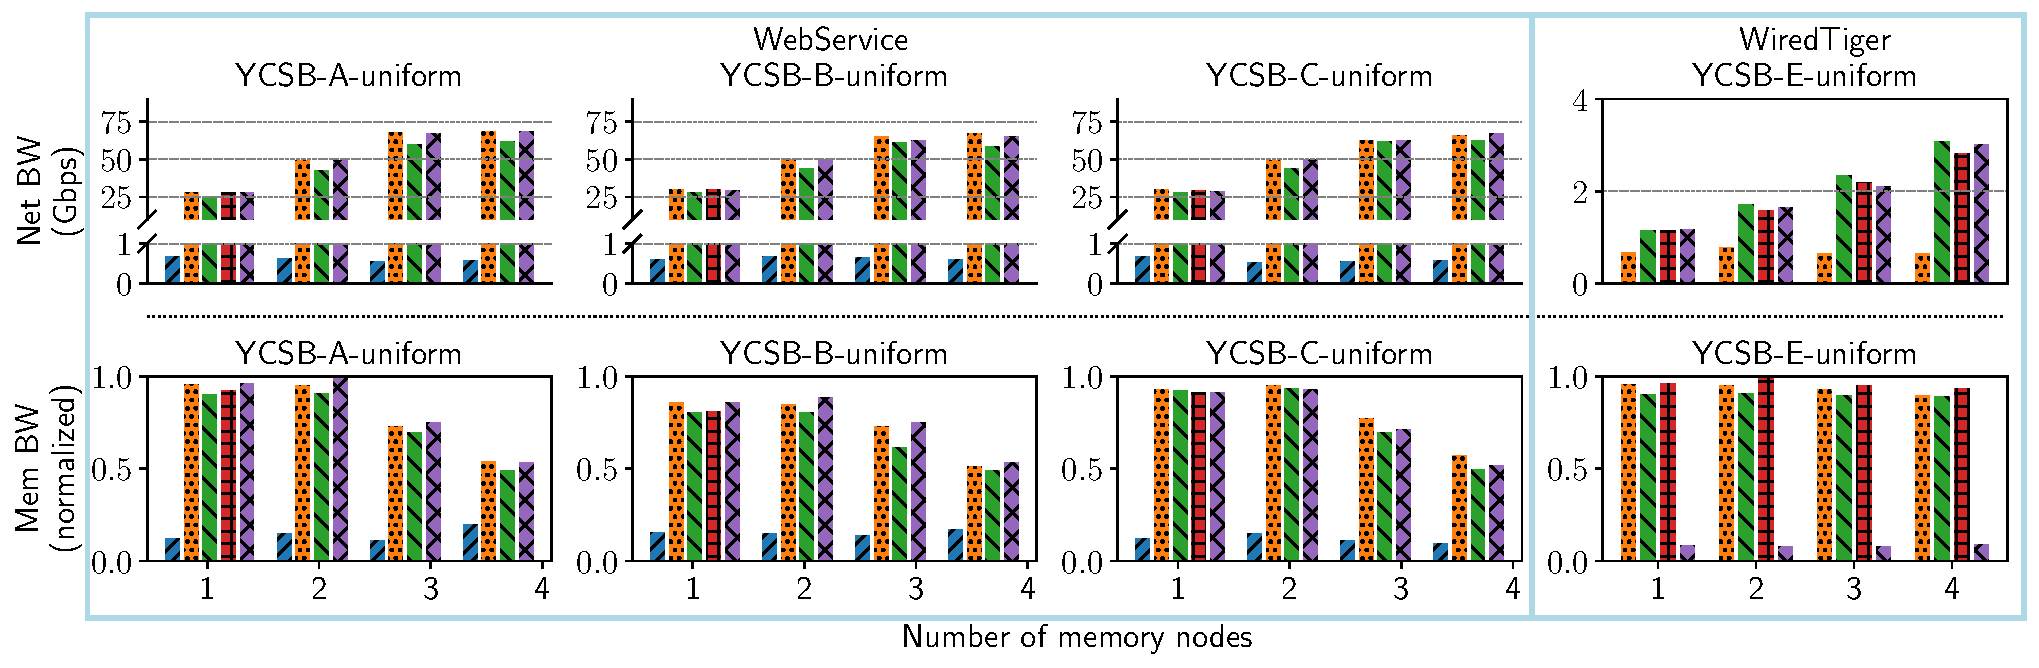
\includegraphics[width=0.9\textwidth]{fig/pulse/network_memory_uniform.pdf}
  \label{fig:sup_eval_perf_e2e_utilization_uniform}
  \vspace{-1.25em}
  %\vspace{-1em}
  \caption{\textbf{Application performance using workload with uniform distribution.}}
  \label{fig:sup_eval_uniform}

\vspace{-1.5em}
\end{figure*}


\subsection{\name Sensitivity Analysis}
\label{ssec:sensitivity}


We evaluate \name's sensitivity to workload characteristics and system parameters: access pattern, data structure modifications, traversal length, allocation policy, and the number of \name memory pipelines. 


\paragraphb{Impact of access pattern}
While our evaluation so far has been confined to Zipfian workloads, we evaluate the impact of skewed access patterns on \name performance for all three applications. Our setup comprises a single $32$GB memory node with a $2$GB CPU node cache. Figure~\ref{fig:sup_cache_friendly} shows caching at the CPU node reduces the number of iterator requests offloaded to the \name accelerator for the skewed (Zipfian) workload, improving \name performance for such workloads by up to $1.33\times$ relative to uniform ones.

\paragraphb{Impact of data structure modifications} Operations that modify data structures can require new memory allocations during traversal. Instead of returning control to the CPU node for allocations, \name populates the scratchpad for every request with a fixed number of pre-allocated memory regions. When a new allocation is initiated at the \name accelerator, it uses a pre-allocated memory region on the scratchpad. If all such regions ($16$ in our implementation) are used up in a single request, the traversal interrupts and returns to the CPU node. \name periodically replenishes pre-allocated entries, ensuring that allocation-triggered traversal interruptions are rare.

We evaluate the impact of data structure modifications in \name (\S\ref{sec:impl}) by increasing the proportion of writes for the WebService application on a single memory node. Figure~\ref{fig:sup_write} shows that as the proportion of writes increases, \name without offloaded allocations experiences higher latencies (up to $1.4\times$) since each new node allocation requires two additional round trips; offloaded allocations reduce the allocation overhead to $<1.1\%$.

\paragraphb{Length of traversal} For simplicity, we evaluate traversal queries on a single linked list with varying numbers of nodes traversed per query. As expected, Fig.~\ref{fig:sup_eval_sensitivity_length} shows that the end-to-end execution latency for a linked list traversal scales linearly with the number of nodes traversed.

\paragraphb{Allocation policy} We find that the allocation policy used for a data structure has a significant impact on application performance specifically for distributed traversals (Figs.~\ref{fig:sup_eval_sensitivity_allocation_latency} and~\ref{fig:sup_eval_sensitivity_allocation_throughput}). We evaluated the WiredTiger and BTrDB workloads (that employ B+-Tree as their underlying data structure) with two allocation policies: one that partitions allocations in a way that ensures all nodes in half the subtree are placed on one memory node and the other half on another, and another that allocates memory uniformly across the two nodes (as in \code{glibc} allocator). The average latency for random allocations is $3.7-10.8\times$ higher than partitioned allocation since it incurs significantly more cross-node traversals. This shows that while uniformly distributed allocations can enable better system-wide resource utilization, it may be preferable to exploit application-specific partitioned allocations for workloads where performance is the primary concern. 

\paragraphb{Number of \name memory pipelines} We evaluate the number of \name memory access pipelines required to saturate \name's memory bandwidth on a single memory node. We used the same linked list as our traversal-length experiment due to its relatively low $\eta$ value ($\sim$$0.06$), which allows us to stress the memory access pipeline without saturating the logic pipeline. Fig.~\ref{fig:sup_eval_sensitivity_core} shows that just $2$ memory pipelines can saturate \name's the per-node memory bandwidth of $25$ GB/s. We note that our $25$ GB/s limit does not match the hardware-specified memory channel bandwidths; this is primarily due to our use of the vendor-supplied memory interconnect IP, required to connect all memory pipelines to all memory channels. Indeed, if we remove the IP and measure memory bandwidth when each memory pipeline is connected to a dedicated memory channel, \name can achieve a memory bandwidth up to $34$ GB/s (shown as \name w/o Interconnect in Fig.~\ref{fig:sup_eval_sensitivity_core}). 

\paragraphb{\name performance with uniform workload} As illustrated in Fig.~\ref{fig:sup_eval_uniform}, while sharing a similar trend as Zipfian distribution, all approaches experience higher latency compared to Zipfian distribution due to the ineffectiveness of caching. \name provides lower (vs. Cache-based, RPC-ARM, and Cache$+$RPC) or comparable (vs. RPC) latency for a single memory node and $2.2$--$29\%$ lower latency (vs. RPC) for multi-memory nodes. 



